\section{Clock Domain Crossing(CDC)}
Clock domain refers to all sequential logic (Flip-Flops, RAMs) that run at one clock frequency. Occasionally multiple clock domains are needed in an FPGA. One needs to be careful while crossing this boundary. The main reason is setup an hold times cannot be guaranteed across clock boundaries. With that, one might lose/corrupt data, or face timing errors.\\
Whenever crossing clock domains, one should be concerned about creating a metastable condition. In general, it's a good idea to use a primitive that is capable of crossing clock domains, such as a Block RAM. Unless one is careful with the register logic and create timing constraints that tell the tools about the exact functionality. Additionally, thr data storage element should be deep enough to cross between the clock domains without losing data. 

\subsection{Basic definitions}
\begin{itemize}
	\item Clock is a signal oscillates between a high and a low state (an analog square wave) and is used like a metronome to coordinate actions of digital circuits.
	\item Rise time refers to the time a clock takes for the rising edge of a pulse to rise from its minimum(10\%) to its maximum(90\%) value.
	\item Fall time refers to the time a clock takes for the falling edge of a pulse to fall from its maximum(90\%) to minimum(10\%) its value.
	\item Settling time is the time required for an output to reach and remain within a given error band following some input stimulus.
	\item Low-to-High-level output (tPLH)
	\item High-to-Low-level output (tPHL)
\end{itemize}




Questions Kumar KJ video\\
\href{https://web.microsoftstream.com/video/e25c7905-a2b7-4a78-a2f2-cbddc09c7e5d?channelId=eaf91042-11bc-4238-8425-dea0e029582d}{VIDEO shared by Ashwini}
 

\subsection{Asynchronous Clocks}
\textbf{Two clocks are called asynchronous if they have do not originate from same clock source and differ in polarity, phase.}


\subsection{Basic definitions for CDC}
\subsubsection{Setup Time} 
\textbf{Setup time} is the amount of time required for the input of a Flip-Flop to be stable before the clock edge comes along.

\subsubsection{Hold Time}
\textbf{Hold time} is the amount of time required for the input of a Flip-Flop to be stable after the clock edge comes along.

\subsubsection{Metastability}
\textbf{Metastability} refers to signals that do not assume stable 0 or 1 states for some duration of time at some point during normal operation of a design. In a multi-clock design, metastability cannot be avoided but the detrimental effects of metastability can be neutralized. In other words, \textbf{Metastability} is a phenomenon that can cause a system failure in digital devices, including FPGAs, when a signal is transferred between circuitry in unrelated or asynchronous clock domains. There's an uncertainty in the logic state of the input data during Metastability condition.

\par A synchronization failure occurs when a signal generated in one clock domain is sampled too close to the rising edge of a clock signal from a second clock domain. Synchronization failure is caused by an output going metastable and not converging to a legal stable state by the time the output must be sampled again.

\subsubsection{Why is metastability a problem?}
A metastable output that traverses additional logic in the receiving clock domain can cause illegal signal values to be propagated throughout the rest of the design.\\
Since the CDC signal can fluctuate for some period of time, the input logic in the receiving clock domain might recognize the logic level of the fluctuating signal to be different values and hence propagate erroneous signals into the receiving clock domain.

\par Every Flip-Flop that is used in any design has a specified setup and hold time. 

\subsubsection{Synchronizers}
A synchronizer is a device that samples an asynchronous signal and outputs a version of the signal that has transitions synchronized to a local or sample clock.

\par There are two scenarios that are possible when passing signals across CDC boundaries:
\begin{itemize}
    \item It is permitted to miss samples that are passed between clock domains. Sometimes it is not necessary to sample every value, but it is important that the sampled values are accurate. Ex. gray code counters.
    \item Every signal passed between clock domains must be sampled. A CDC signal must be properly recognized or acknowledged before a change is permitted on the CDC signal.
\end{itemize}
In both of these scenarios, the CDC signals will require some form of synchronization into the receiving clock domain.

\subsubsection{Two Flip-Flop synchronizer}
The simplest and most common synchronizer used by digital designers is a two-Flip-Flop synchronizer. The first Flip-Flop samples the asynchronous input signal into the new clock domain and waits for a full clock cycle to permit any metastability on the stage-1 output signal to decay, then the stage-1 signal is sampled by the same clock into a second stage Flip-Flop, with the intended goal that the stage-2 signal is now a stable and valid signal synchronized and ready for distribution within
the new clock domain. Both the Flip-Flops run on the destination clock.

\subsubsection{Mean Time Before Failure (MTBF)}
It is theoretically possible for the stage-1 signal to still be sufficiently metastable by the time the signal is clocked into the second stage to cause the stage-2 output signal to also go metastable. Mean time between synchronization failures (MTBF) Definition. 

The calculation of the probability of the (MTBF) depends on: 
\begin{itemize}
    \item clock frequencies of the input
    \item clock the synchronizing Flip-Flops
    \item the sample clock frequency (how fast are signals being sampled into the receiving clock domain) and
    \item the data change frequency (how fast is the data changing that crosses the CDC boundary)
\end{itemize}

For most synchronization applications, the two Flip-Flop synchronizer is sufficient to remove all likely metastability.

It is important to run a calculation of the MTBF for any signal crossing a CDC boundary. Failure in this case means that the signal passed to a synchronizing Flip-Flop, goes metastable on the first stage synchronizer Flip-Flop, and continues to be metastable one cycle later when it is sampled into the second stage synchronizer Flip-Flop. 

Since the signal did not settle to a known value after one clock cycle, the signal could still be metastable when sampled and passed to the receiving clock domain, causing potential failures to the corresponding logic.

Larger MTBF numbers indicate longer periods of time between potential failures, while smaller MTBF numbers indicate that metastability could happen frequently, similarly causing failures within the design.

\[MTBF = 1/(f_{clk} * f_{data} * X )\]

where,\\
X = other factors,\\
\(f_{clk}\) : Synchronizing clock frequency,\\
\(f_{data}\) : Data changing frequency.

\par Failures occur more frequently in designs with higher speeds, or when the sampled data changes are more frequent.


\subsubsection{Three Flip-Flop synchronizer}
For some very high speed designs, the MTBF of a two-flop synchronizer is too short and a third flop is added to increase the MTBF to a satisfactory duration of time. 

\par Synchronizing signals from the sending clock domain is necessary. Also, synchronizing signals into the receiving clock domain is necessary before being passed to a CDC boundary. 

\par The synchronization of signals from the sending clock domain reduces the number of edges that can be sampled in the receiving clock domain, effectively reducing the data-change frequency and hence, increasing MTBF.


\subsection{Synchronizing fast signals into slow clock domains}
One issue associated with synchronizers is the possibility that a signal from a sending clock domain might change values twice before it can be sampled, or might be too close to the sampling edges of a slower clock domain. \\ When missed samples are not allowed, there are two general approaches to the problem:
\begin{itemize}
    \item An open-loop solution to ensure that signals are captured without acknowledgment.
    \item A closed-loop solution that requires acknowledgement of receipt of the signal that crosses a CDC boundary.
\end{itemize}

\subsubsection{The "three edge" guideline}
According to Mark Litterick, when passing one CDC signal between clock domains through a two-flip-flop synchronizer, the CDC signal must be wider than 1.5 times the cycle width of the receiving domain clock period.\\ \centerline{\textbf{"Input data values must be stable for three destination clock edges."}}

The "three edge" requirement actually applies to both open-loop and closed-loop solutions, but the closed-loop solution implementations already follow the requirement.

Issues while sending fast signals into slow clock domains: 
\begin{itemize}
	\item The CDC signal could have a transition between the rising edges of a slower clock and will not be captured into the slower clock domain.
	\item The CDC signal that is slightly wider than the period of the receiving clock frequency might change too close to the two rising clock edges of
	the receiving clock domain making setup and hold violations.
\end{itemize}

\subsubsection{Open loop solution}
There is a requirement for reliable signal passing between clock domains. One solution to resolve this issue is to use a faster clock domain frequency 1.5 times (or more) than that of the slower clock domain frequency.\\
Since the faster clock signal might sample the slower clock domain signal one or more times.\\
This solution can be used when relative clock frequencies are fixed and properly analyzed.

\paragraph{Advantage}
The open loop solution is the fastest way to pass signals across CDC Boundaries that does not require acknowledgement of the received signals.

\paragraph{Disadvantage}
Another engineer might mistake the solution for a general purpose solution, or the design requirements
might change and an engineer might fail to reanalyze the original open loop solution. This problem can be minimized by adding a SystemVerilog Assertion to the model to detect if the input pulse ever fails to exceed the "three edges" design requirement.


\subsubsection{Closed loop solution}
In closed loop solution,  will send an enabling control signal and synchronize it into the new clock domain and then pass the synchronized signal back through another synchronizer to the sending clock domain as acknowledge signal.

The closed loop solution is a more general solution and can be used in a variety of designs in contrast to open loop solution.

\paragraph{Advantage} Synchronizing a feedback signal is a very safe technique to acknowledge that the first control signal was recognized and sampled into the new clock domain.

\paragraph{Disadvantage} There is potentially considerable delay associated with synchronizing control signals in both directions before allowing the control signal to change.


\subsection{Passing multiple signals between clock domains}
A frequent mistake made by engineers when working on multi-clock designs is passing multiple CDC bits required in the same transaction from one clock domain to another and overlooking the importance of the synchronized sampling of the CDC bits.

\par The problem is that multiple signals that are synchronized to one clock will experience small data changing skews that can occasionally be sampled on different rising clock edges in a second clock domain. Multi-bit CDC strategies must be employed to avoid skewed sampling of the multi-bit value.

\subsubsection{Multi-bit CDC strategies}
There are 3 main categories of the multi-bit CDC strategies.
\begin{itemize}
	\item Multi-bit signal consolidation
	\item Multi-cycle path formulations
	\item Passing multiple CDC bits using gray codes
\end{itemize}

\subsubsection{Multi-bit signal consolidation}
Where possible, consolidate multiple CDC signals into a 1bit CDC signal. If the order or alignment of the control signals is significant, care must be taken to correctly pass the signals into the new clock domain.

\subsubsection{Multi-cycle path(MCP) formulations}
An MCP formulation refers to sending an unsynchronized data to a receiving clock domain paired with a synchronized control signal.\\
The data and control signals are sent simultaneously allowing the data to setup on the inputs of the destination register while the control signal is synchronized for two receiving clock cycles before it arrives at the load input of the destination register.
\paragraph{Advantages}
\begin{itemize}
\item The sending clock domain is not required to calculate the appropriate pulse width to send between clock domains.
\item The sending clock domain is only required to toggle an enable into the receiving clock domain to indicate that data has been passed and is ready to be loaded. The enable signal is not required to return to its initial logic level.
\end{itemize}
The receiving clock domain is not
allowed to sample the multi-bit CDC signals until the synchronized enable passes through synchronization and arrives at the receiving register.

The unsynchronized data word is passed directly to the receiving clock domain and held for multiple receiving clock cycles, allowing an enable signal to be synchronized and recognized into the receiving clock domain before permitting the unsynchronized data word to change. This is why, this strategy is called Multi-Cycle Path Formulation.

\par As the unsynchronized data is passed and held stable for multiple clock cycles before being sampled, there is no danger of Metastability.


\paragraph{MCP formulation using a synchronized enable pulse}
This method employs a toggling enable signal that is passed to a synchronized pulse generator to indicate that the unsynchronized multi-cycle data word can be captured on the next receiving clock edge.

A key feature of this synchronized enable pulse generation is that the polarity of the input signal does not matter.

\[*******************Revisit*******\]


Multi-Cycle Path (MCP) formulations can be used to address problems related to passing multiple CDC signals. THere are two types of MCP formulations that can be used to fix this problem:
\begin{enumerate}
	\item Closed-loop - MCP formulation with feedback
	\item Closed-loop - MCP formulation with acknowledge feedback
\end{enumerate}

\paragraph{Closed-loop - MCP formulation with feedback}
An important technique while using an MCP formulation is to pass the enable signal back to the sending clock domain as an acknowledge signal.\\
This is an automatic feedback path that assumes that the receiving clock domain will always be ready for the next data word synchronized through an MCP formulation.

\paragraph{Closed-loop - MCP formulation with acknowledge feedback}

Another important technique while using an MCP formulation is to pass the enable signal back to the sending clock domain as an acknowledge signal only after the receiving clock domain acknowledges the receipt of the data with a bload pulse.


\subsubsection{Passing multiple CDC bits using gray codes}
One characteristic of binary counters is that half of all sequential binary incrementing operations require that two or more counter bits must change.
In contrast to binary counters, Gray codes only allow one bit to change for each clock transition, eliminating the problem associated with trying to synchronize multiple changing CDC bits across a clock domain.

This in turn reduces chances of errors due to less number of bit changes per transaction.

\subsubsection{Additional multi-bit CDC techniques}
Standard FIFOs are used to pass data and control signals between clock domains. FIFO techniques can be used to address problems related to passing multiple CDC signals. FIFO strategies that act as closed loop solutions to this problem are:
\begin{enumerate}
	\item Asynchronous FIFO implementation
	\item 1-deep / 2-register FIFO implementation
\end{enumerate}

\paragraph{Asynchronous FIFO implementation}
Passing multiple bits, whether data bits or control bits, can be done through an asynchronous FIFO. An asynchronous FIFO is a shared memory or register buffer where data is inserted from the write clock domain and data is removed from the read clock domain. Since both sender and receiver operate within their own respective clock domains, using a dual-port buffer, such as a FIFO, is a safe way to pass multi-bit values between clock domains.


A standard asynchronous FIFO device allows multiple data or control words to be inserted as long as the FIFO is not full, and the receiver and then extract multiple data or control words when convenient as long as the FIFO is not empty.


\paragraph{1-deep / 2-register FIFO implementation}

On reset, both pointers are cleared and the FIFO is empty and hence the FIFO is not full. We use the inverted not-full condition to indicate that the FIFO is ready to receive a data or control word (wrdy is high). After a data or control word is put into the FIFO (using wput), the wptr toggles and the FIFO becomes full, or in other words, the wrdy signal goes low, which also disables the ability to toggle the wptr and therefore also disables the ability to put another word into the 2-register FIFO until the first word is removed from the FIFO by the receiving clock-domain logic.

\par What is especially interesting about this design is that the wptr is now pointing to the second location in the 2-register FIFO, so when the FIFO does again become ready (when wrdy is high), the wptr is already pointing to the next location to write.

\par The same concept is replicated on receiving side of the FIFO. When a data or control word is
written into the FIFO, the FIFO becomes not empty. We use the inverted not-empty condition to
indicate that the FIFO is has a data or control word that is ready to be received (rrdy is high).

\par By using two registers to store the multi-bit CDC values, we are able to remove one clock cycle from the send MCP formulation and another cycle from the acknowledge feedback path.

\subsection{Naming conventions \& design partitioning}
Naming conventions help to ensure good team communication and also facilitate the use of
scripting languages to gather and group all signals in a design that are associated with a particular
clock. Good design partitioning can significantly reduce the effort to synthesize and verify the
timing of a multi-clock design. 

There are two approaches to address potential CDC problems: (1) verify that the design meets
qualified CDC rules, (2) avoid the problem. Both approaches are valuable and should be used to
ensure an error-free design.

The problem could be avoided by employing a few good coding guidelines.

\subsubsection{Clock \& signal naming conventions}
Guideline: Use a clock naming convention to identify  the clock source of every signal in a design.
One proven naming convention requires that a leading prefix character be used to identify the
various asynchronous clock domains. Examples included: uClk for the microprocessor clock, vClk for the video clock and dClk for the display clock.
Each signal is then synchronized to one of the clock domains in the design and each signal-name
is labeled with a prefix character to identify the clock domain used to generate that signal.

\subsubsection{Multi-clock / multi-source modules with no naming convention}
If your team does not using any particular clock-oriented signal naming convention and if
modules are allowed to have multiple clock inputs, there is always the danger that the CDC
analysis tool might not be setup correctly and it is easy to miss bad CDC design practices.

\subsubsection{Timing verification for each clock domain}
To verify the timing of any design, one must verify the that timing is met for each clock domain
in a design. Although tools have improved over the past decade to help automate the analysis and
verification of signals in separate clock domains, it is still a good practice to approach multiclock
design using good partitioning and naming conventions.
By partitioning a design to permit only one clock per module, static timing analysis becomes a
significantly easier task for each domain in the design.

\subsubsection{Clock oriented design partitioning}
Some of the simplest and best design partitioning methodologies are implemented using design partitioning at clock boundaries.
guidelines
\begin{itemize}
	\item Only allow one clock per module except the top module
	\item Partition the design blocks into one-clock modules
	\item Create synchronizer modules to pass signals from one clock domain into another clock domain and only allow one clock per synchronizer module.
\end{itemize}

Timing analysis of clock-partitioned modules

\subsubsection{Partitioning with MCP formulations}
Partitioning a design at clock boundaries into separate design blocks and synchronizer blocks works well most of the time, but if multiple signals need to be passed between clock domains using an MCP formulation, then some of the signals that are passed to a design block may come from a different clock domain.

\par Design blocks with asynchronous inputs can still be easily timed if a clock based naming convention has been used for the signals in the design. Before performing STA on the design block in question, simply exclude the asynchronous inputs from the analysis. With this, only the inputs to the synchronizers and MCP formulation data paths require "set\_false\_path" commands.

\subsection{Multi-clock gate-level simulation issues}

Following issues faced during Multi-clock gate-level simulations: 
\begin{itemize}
	\item 
\end{itemize}
Synchronizer gate-level CDC simulation issue: Digital simulation models typically generate X's when synchronizers recognize setup and hold time violations on CDC signals. 

\subsubsection{Strategies to remove X-propagation from gate-level simulations}
There exists an unwanted propagation of X's every time a signal violates a setup or hold time on the first stage of the synchronizer.
Below are some of the strategies that have
been considered to address the X-propagation problem: 
\begin{itemize}
	\item Simulator command to turn off timing checks (Not Recommended as this method ignores the desired timing checks for the rest of the design.)
	\item Change flip-flop setup and hold times to 0 (Simulation Libraries)
	\item Use multiple SDF files (The first SDF file can have all the actual delays, including accurate setup and hold times, for the entire design. The second SDF file with only the first stage flip-flops included can have the setup and hold times are set to 0.) 
\end{itemize}

\subsection{Summary}
Clock Domain Crossing (CDC) errors can cause serious design failures. These expensive failures can be avoided by following a few critical guidelines and using well established verification techniques.

\subsubsection{Recommended 1-bit CDC techniques}
When passing one bit between clock domains:
\begin{itemize}
	\item register the signal in the sending clock domain to remove combinational settling
	\item synchronize the signal into the receiving clock domain. A Multi-Cycle Path (MCP) formulation may be necessary
\end{itemize}

\subsubsection{Recommended multi-bit CDC techniques}
When passing multiple control or data signals between clock domains, use one of the following strategies:
\begin{itemize}
	\item Consolidate - first attempt to combine multiple signals into a 1-bit representation in the sending clock domain before synchronizing the signal into the receiving domain
	\item Use Multi-Cycle Path (MCP) formulations to pass multiple signals across clock domains
	\item Use FIFOs to pass multi-bit buses, either data or control buses
	\item Use gray code counters
\end{itemize}

\subsubsection{Recommended naming conventions and design partitioning}
\begin{itemize}
	\item Use a clock-based naming convention 
	\item As much as possible, partition the design sub-blocks into completely synchronous 1-clock designs
\end{itemize}



\subsubsection{Recommended solutions to multi-clock gate-level CDC simulations}
There are multiple useful solutions to the CDC X-propagation simulation issues during gate-level
simulation:
\begin{itemize}
	\item Use a Synopsys switch to generate 0-setup and 0-hold times for first stage flip-flops on synchronizers. Works okay with Synopsys tools only
	\item Use multiple SDF files - good technique described later in this section
	\item Vendor provides a synchronizer cell and appropriate SDF tools - great solution if your ASIC or FPGA vendor provides the models and tools (very few do - ask you ASIC \& FPGA vendors to support this feature)
	\item Use creative SystemVerilog models to model synchronization problems
\end{itemize}

\subsection{Reference for CDC Section}
Clock Domain Crossing (CDC) Design \& Verification Techniques Using SystemVerilog\\
Clifford E. Cummings\\
Sunburst Design, Inc.\\
Important design considerations require that multi-clock designs be carefully constructed at
Clock Domain Crossing (CDC) boundaries. This paper details some of the latest strategies and
best known methods to address passing of one and multiple signals across a CDC boundary.
Included in the paper are techniques related to CDC verification and an interesting 2-deep FIFO
design for passing multiple control signals between clock domains. Although the design methods
described in the paper can be generally implemented using any HDL, the examples are shown
using efficient SystemVerilog techniques.

\subsection{Clock Domain Crossing from NANDLAND}


\subsubsection{Case I : Crossing from Slow to Fast domain}
This is the first case of getting a metastable condition while crossing clock domains. This specific condition refers to the crossing from slow to fast clock domain. There's a simple solution to overcome this condition. One can add 2 flip flops with a clock of faster clock \textbf{(Synchronizer)} to get a stable input for the FPGA as shown in fig \figref{SlowToFastCDC}. This is also used to bring non-clocked data into the FPGA from an external source.

\begin{figure}[H]
	\begin{center}
		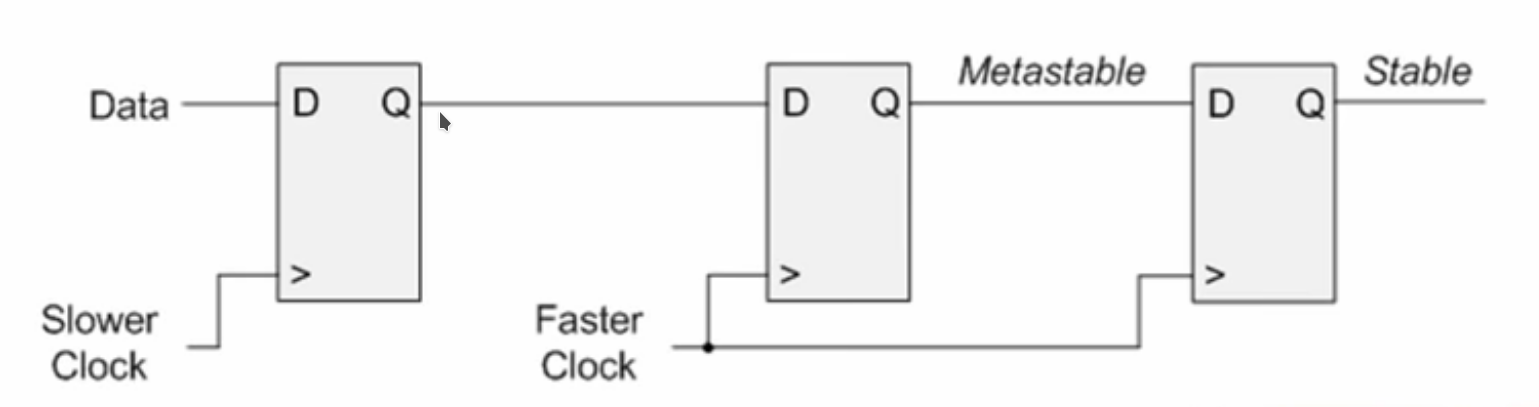
\includegraphics[width=5in]{images/SlowToFastCDC.png}
		\caption{Crossing from Slow to Fast domain}
		\label{SlowToFastCDC}
	\end{center}
\end{figure}


\subsubsection{Case II : Crossing from Fast to Slow domain}
This is the second case of getting a metastable condition while crossing clock domains. This specific condition refers to the crossing from fast to slow clock domain. There's a simple solution to overcome this condition. One can stretch the faster clock pulse for a duration in whcih the slower clock can definitely detect it as shown in the sample clocks of fig \figref{FastToSlowCDC}. 

\begin{figure}[H]
	\begin{center}
		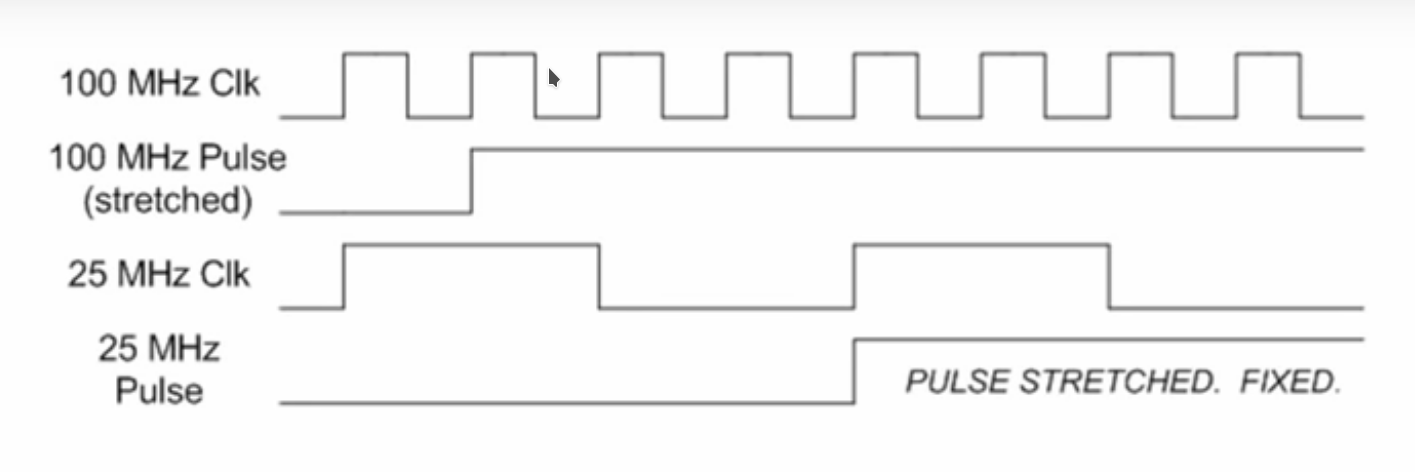
\includegraphics[width=5in]{images/FastToSlowCDC.png}
		\caption{Crossing from Fast to Slow domain}
		\label{FastToSlowCDC}
	\end{center}
\end{figure}

\subsubsection{Case III : Crossing with Streaming Data}
This is the third case of getting a metastable condition while crossing clock domains. This specific condition refers to the crossing with streaming data. There's a simple solution to overcome this condition. The best solution to ensure a stable condition over Metastability is using FIFOs.

\par \textbf{FIFO} stands for First In First Out. It usually comprises of an input data, an output data, width, and depth of the FIFO. FIFOs are made up of either registers or BRAMs. Register based FIFOs are usually smaller when compared with the BRAM based FIFOs. FIFOs are synchronous on both input and output sides of FIFO. FIFOs can use an Independent or a common clock for the input and output. There are two checklists for a FIFO: Never read from an empty FIFO and Never write to a Full FIFO. Don't go beyond overflow and underflow. 


\begin{figure}[H]
	\begin{center}
		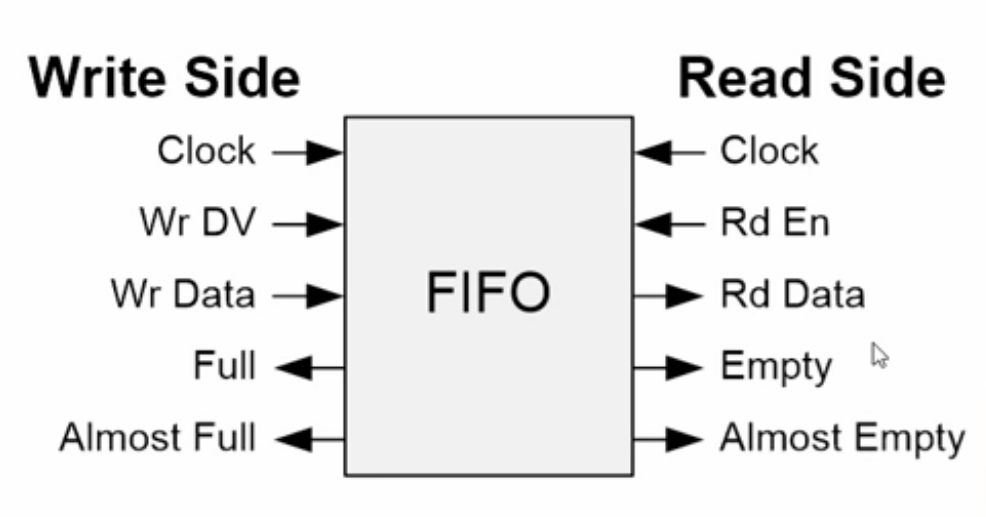
\includegraphics[width=5in]{images/FIFO.png}
		\caption{Signals of FIFO}
		\label{FIFO}
	\end{center}
\end{figure}

\subsubsection{Timing Errors}
Design tools throw timing errors when there are multiple clock domains. One has to know the reason, the source and the solution of each and every timing error. Timing constraints are written in order to overcome/neglect these timing errors. The place and route score should be zero in order to achieve the stable system.

\subsubsection{Propogation Delay}
Propagation Delay is the time taken for a signal to travel from a source Flip-flop to a destination Flip-flop. Voltage in wires take time to travel. This distance between the Flip-flops due to routing and placement results in a propagation delay.
